\documentclass[sigconf,review,anonymous]{acmart}

\usepackage{amsmath}
\usepackage{algorithm}
\usepackage[noend]{algpseudocode}
\usepackage{booktabs}
\usepackage{multirow}
\usepackage{pgfplots}
\usepackage{placeins}
\usepackage{siunitx}
\usepackage{tikz}
\usepackage{xspace}
\usetikzlibrary{arrows.meta,decorations.pathreplacing,fit,positioning,shapes.geometric}
\usepgfplotslibrary{groupplots}
\pgfplotsset{compat=1.18}

\setcopyright{none}
\settopmatter{printacmref=false,printccs=false,printfolios=true}
\renewcommand\footnotetextcopyrightpermission[1]{}

\newcommand{\system}{\textsc{GraphWeft}\xspace}
\newcommand{\sharedexpand}{\textsc{Vertex\allowbreak Share}\xspace}
\newcommand{\coalescedgather}{\textsc{Aligned\allowbreak Gather}\xspace}
\newcommand{\drafttodo}[1]{\textcolor{red!75!black}{\textbf{[TODO: #1]}}}
\newcommand{\preliminary}[1]{\textcolor{blue!60!black}{#1}}
\newcommand{\querymask}{\mathcal{M}}
\newcommand{\frontier}{\mathcal{F}}

\title{GraphWeft: Mitigating Memory-Access Overhead for Concurrent Graph Query Processing on GPUs}

\acmConference[SIGMOD '27]{ACM SIGMOD International Conference on Management of Data}{June 13--19, 2027}{Huntington Beach, CA, USA}
\acmYear{2027}
\copyrightyear{2027}

\author{Anonymous Author(s)}
\affiliation{\institution{Anonymous Institution}}

\begin{abstract}
Concurrent graph query processing evaluates many analytics over the same graph, but executing them independently repeatedly accesses common neighborhoods and incurs irregular accesses to query-specific state.
This problem is particularly costly on GPUs, where graph computation is often limited by exposed memory-access latency; existing concurrent graph systems primarily increase parallelism or align traversal phases without treating memory access as a unified optimization target.
We present \system, a concurrent graph query engine based on a simple principle: share repeated accesses and regularize the remainder.
\system combines exact query-aware vertex sharing to reduce neighborhood-access count, access-efficient aggregation to lower the cost of the remaining state accesses, and sharing-aware scheduling to expose more reusable work across queries.
\drafttodo{Replace this sentence with the final end-to-end headline: fixed policy, current code, at least three algorithms, all graphs, and planner cost included.}
\end{abstract}

\ccsdesc[500]{Information systems~Graph-based database models}
\ccsdesc[500]{Information systems~Data analytics}
\ccsdesc[300]{Computing methodologies~Massively parallel algorithms}
\keywords{concurrent graph queries, graph analytics, GPU, work sharing, memory access}

\begin{document}
\maketitle

\section{Introduction}

Graph services increasingly evaluate many analytical queries over the same graph.  A routing service answers paths from different origins, a social-network backend evaluates reachability or influence for many users, and an analyst submits a window of the same graph algorithm with different sources or parameters.  We refer to this workload as \emph{concurrent graph query processing} (CGQ).  Unlike a single graph analytic, a CGQ workload contains repeated access to one largely static topology while retaining independent query states and results.  Its systems objective is therefore to complete the query window efficiently without changing any constituent query.

GPUs are attractive for CGQ because they provide high memory bandwidth and parallel processing capacity.  Yet graph computation is dominated by data movement: adjacency lists are irregular, active vertices change from one iteration to the next, and query states are scattered across the graph.  Concurrency does not remove this bottleneck.  When two queries reach the same vertex, independent execution accesses the same neighbor list twice; when their traversals diverge, executing them together can add contention without reuse.  In our pilot profiles, exposed data-access stalls account for 43.1--59.8\% of issue stalls in representative iterations even though achieved bandwidth ranges from only 31.0--62.0\% of peak.  These measurements point to memory-access latency, rather than insufficient arithmetic, as the central bottleneck for our target workload.

Recent database graph systems address important but different limitations.  TGraph provides a tensor-centric model that hides accelerator-specific details~\cite{zhang_tgraph_2025}; CGgraph improves out-of-memory processing and CPU--GPU cooperation~\cite{cui_cggraph_2024}; and CompressGraph reuses repeated neighbor sequences through direct processing on a compressed representation~\cite{chen_compressgraph_2023}.  These systems primarily optimize one graph analytic at a time.  Concurrent graph systems instead share computation or coordinate multiple queries: \textsc{iBFS} fuses BFS instances on GPUs~\cite{liu_ibfs_2016}, while \textsc{Glign} groups and delays traversals to align expensive phases~\cite{yin_glign_2022}.  Apart from specialized BFS execution, however, existing work does not systematically organize general CGQ execution around its memory-access bottleneck.

Our key observation is that concurrency creates both the problem and the opportunity.  It increases the number of active states, but it also exposes repeated neighborhood accesses and a new regular dimension across queries.  We can therefore mitigate memory-access overhead in two complementary ways: \emph{reduce the number of accesses} by sharing a neighborhood among exactly the queries that currently need it, and \emph{reduce the effective cost of the remaining accesses} by processing query states in a regular order.  Query scheduling provides a third lever: it changes when traversals reach the same graph region and hence how much access reuse is available.

Figure~\ref{fig:core-idea} summarizes this principle: \emph{share repeated accesses and regularize the remainder}.  This is a workload-level view rather than a GPU execution detail.  It first asks which graph data and query states are logically reusable, then maps the resulting computation to the hardware in Section~\ref{sec:implementation}.

\begin{figure}[t]
  \centering
  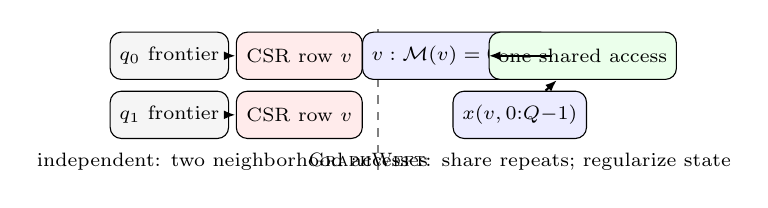
\begin{tikzpicture}[
      font=\scriptsize,
      box/.style={draw, rounded corners, align=center, minimum height=6mm},
      arrow/.style={-{Latex[length=1.5mm]}, thick},
      cost/.style={font=\scriptsize, align=center}
    ]
    \node[box, fill=gray!8] (i0) at (0,0.7) {$q_0$ frontier};
    \node[box, fill=gray!8] (i1) at (0,-0.05) {$q_1$ frontier};
    \node[box, fill=red!8, minimum width=16mm] (r0) at (1.65,0.7) {CSR row $v$};
    \node[box, fill=red!8, minimum width=16mm] (r1) at (1.65,-0.05) {CSR row $v$};
    \draw[arrow] (i0) -- (r0);
    \draw[arrow] (i1) -- (r1);
    \node[cost] at (0.8,-0.65) {independent: two neighborhood accesses};

    \draw[dashed, gray] (2.65,-0.75) -- (2.65,1.05);

    \node[box, fill=blue!8] (mask) at (3.65,0.7) {$v: \querymask(v)=0011_2$};
    \node[box, fill=green!8] (row) at (5.25,0.7) {one shared access};
    \node[box, fill=blue!8] (state) at (4.45,-0.05) {$x(v,0{:}Q{-}1)$};
    \draw[arrow] (mask) -- (row);
    \draw[arrow] (state) -- (row);
    \node[cost] at (4.45,-0.65) {\system: share repeats; regularize state};
  \end{tikzpicture}
  \caption{The core principle: share repeated accesses and regularize the remainder.  \system represents exact query overlap at a vertex, accesses its neighborhood once, and keeps the associated query states together.}
  \Description{Two independent query frontiers each access the same adjacency row. GraphWeft combines them into one vertex with an exact query mask, one shared neighborhood access, and a contiguous row of query values.}
  \label{fig:core-idea}
\end{figure}


Realizing this opportunity raises three challenges.

\paragraph{C1: Reuse must preserve query semantics.}
Two queries may visit the same vertex at different logical levels or with different values.  A query-oblivious union can access a neighbor list once but may apply unrelated queries to it, replacing redundant memory accesses with false computation.  The system must expose exact, iteration-local overlap while preserving independent values and convergence state.

\paragraph{C2: Access reduction and access regularity have different win regions.}
Sharing an active vertex reduces neighborhood accesses when frontiers are sparse and overlapping.  During broad phases, however, irregular updates to many query states can dominate, and a destination-oriented traversal with regular query-state access may be preferable even if it examines more edges.  No single traversal strategy minimizes memory overhead across all graphs and iterations.

\paragraph{C3: Shareability changes over time.}
Queries that eventually visit similar regions may reach them in different iterations.  Grouping and start-time alignment can increase simultaneous overlap, but excessive delay or planning cost can erase the benefit.  Coordination must therefore improve realized access reuse rather than optimize a static source-similarity score alone.

We present \system, a CGQ engine for a GPU-resident graph.  Its thesis is that \emph{CGQ performance can be improved by treating memory-access overhead as a unified design objective across query representation, graph traversal, and scheduling}.  \system uses exact per-vertex query masks to represent current overlap.  \sharedexpand shares each active vertex's neighborhood among only the queries named by its mask, reducing topology accesses.  \coalescedgather processes the remaining query states in a vertex-major order, reducing their effective access cost during broad phases.  A phase-aware scheduler groups and offsets queries to expose more simultaneous vertex overlap, while an adaptive selector chooses the traversal strategy from exact runtime state.  Approximate scheduling may miss an optimization opportunity, but it cannot change a query answer.

This paper makes four contributions:

\begin{itemize}
  \item We formulate GPU-based CGQ as a memory-access problem and decompose its overhead into repeated topology accesses and the effective cost of query-state accesses.  Pilot measurements connect both terms to observed execution behavior (Section~\ref{sec:background}).
  \item We develop an exact vertex-sharing computation model and two complementary traversal strategies: \sharedexpand reduces repeated neighborhood accesses, while \coalescedgather organizes broad query-state aggregation for efficient access.  Both support typed BFS, SSSP, and widest-path state rather than only BFS status bits (Section~\ref{sec:design}).
  \item We design a sharing-aware scheduler that estimates pairwise traversal phases, forms query batches, and selects bounded start offsets to increase realized vertex sharing.  Runtime decisions use exact query state, so prediction quality affects performance but not correctness (Sections~\ref{sec:overview} and~\ref{sec:planner}).
  \item We implement these ideas in a 7.6-KLoC C++17/CUDA prototype and define an evaluation that measures end-to-end CGQ throughput, memory-access reduction, component contributions, scheduling quality, scalability, and overhead (Sections~\ref{sec:implementation} and~\ref{sec:evaluation}).
\end{itemize}

Current results are preliminary and delimit the remaining work.  For all-push BFS with 128 queries and 32 resident slots, online grouping and offsets reduce union-edge accesses by 15.5--64.4\% and improve batch execution by $1.15\times$--$2.31\times$ on six graphs.  The current fixed-$Q{=}64$ hybrid path, however, reaches only $0.49\times$ the geometric-mean throughput of \textsc{iBFS} on four graphs.  Section~\ref{sec:evaluation} therefore treats fixed-policy performance, the traversal selector, and the same-engine \textsc{iBFS}/\textsc{Glign} decomposition as gating evidence rather than hiding the gap behind favorable configurations.

\section{CGQ Model and Motivation}
\label{sec:background}

Following the style of recent database graph systems, this section first defines the computation model and then derives the design from measured workload properties.  The low-level GPU mapping is deferred to Section~\ref{sec:implementation}.

\subsection{Concurrent Graph Query Model}

Let $G=(V,E)$ be a directed graph stored once in device memory.  A query window contains $N$ source-based iterative queries over $G$.  At most $Q\leq64$ queries are resident in one batch; larger windows are divided into batches.  Query $q$ maintains a value $x_q(v)$ for every vertex and a frontier $\frontier_q^{\ell}$ at logical level $\ell$.  BFS stores distance and discovery state, SSSP stores weighted distance, and widest-path traversal stores a bottleneck value.  Correct CGQ execution must return the same value vector for every query as independent level-synchronous execution.

At global iteration $t$, query $q$ is either inactive or at logical level $\ell_q(t)$.  We define its exact union frontier and the query membership of each active vertex as
\begin{align}
  U_t &= \bigcup_{q\text{ active}} \frontier_q^{\ell_q(t)}, \\
  \querymask_t(v) &= \{q \mid v\in\frontier_q^{\ell_q(t)}\}.
\end{align}
$U_t$ identifies neighborhoods that may be reused; $\querymask_t(v)$ identifies exactly which queries may reuse the neighborhood of $v$.  A compact word represents the membership set for the current prototype, but the model itself is independent of that representation.

We target a closed query window over one static, GPU-resident graph.  Query sources may differ and queries may start at different global iterations.  Dynamic graphs, continuous arrival control, and multi-GPU partitioning are outside the central claim and are discussed in Section~\ref{sec:limitations}.

\subsection{Optimization Objective}

A CGQ system makes three coupled decisions for a query window $W$.  It partitions the queries into resident batches $\mathcal{B}$, assigns each query a bounded start offset $o_q$, and selects an access strategy $a_t$ at every global iteration.  We denote a complete choice by
\begin{equation}
  \Pi(W)=\langle\mathcal{B},\{o_q\}_{q\in W},\{a_t\}_{t\geq 0}\rangle.
\end{equation}
The batch and offsets determine which query frontiers coexist; the iteration strategy determines how the resulting graph and state work is accessed.  Optimizing any one choice in isolation can be misleading: a good strategy cannot share queries placed in different batches, while aggressive alignment can add more delay than the saved execution time.

Our primary objective is to minimize query-window completion time
\begin{equation}
  T(W,\Pi)=T_{\mathrm{schedule}}+T_{\mathrm{execute}}
  \label{eq:window-objective}
\end{equation}
subject to a resident-memory budget and per-query result equivalence with independent execution.  Query-dependent grouping, offsets, feature collection, and strategy selection are therefore online costs.  Reusable graph analysis is reported separately with its construction, storage, load, and break-even costs.  P50 and P95 query latency complement the window objective so that delaying a query to create sharing cannot appear free.

The system must select one policy without knowing the fastest alternative in advance.  Per-graph or per-query hindsight may characterize an upper bound, but it is not a deployable configuration.  The main evaluation consequently freezes the scheduling and strategy-selection policy and reports an oracle only as diagnostic evidence.

\subsection{A Memory-Access View of CGQ}

Independent frontier expansion accesses
\begin{equation}
  E_{\mathrm{ind}}(t)=
    \sum_q\sum_{v\in\frontier_q^{\ell_q(t)}}\deg^+(v)
\end{equation}
adjacency entries.  If every active vertex is processed once for the entire batch, the topology-access count becomes
\begin{equation}
  E_{\mathrm{union}}(t)=\sum_{v\in U_t}\deg^+(v).
\end{equation}
The normalized neighborhood-sharing opportunity is
\begin{equation}
  S_{\mathrm{share}}(t)=1-\frac{E_{\mathrm{union}}(t)}
                                    {E_{\mathrm{ind}}(t)}.
\end{equation}
It is zero for disjoint frontiers and approaches one when many queries simultaneously contain the same high-degree vertices.

Sharing the topology does not remove query-specific relaxations.  Their logical count is
\begin{equation}
  E_{\mathrm{pair}}(t)=
    \sum_{v\in U_t}\deg^+(v)\,\mathrm{popcount}(\querymask_t(v)).
\end{equation}
This distinction prevents an apparent reduction in adjacency access from hiding false query--edge work.  $E_{\mathrm{union}}$ captures how many graph entries need to be fetched, while $E_{\mathrm{pair}}$ bounds how much query-specific state must be examined.

Memory overhead is not determined by access count alone.  The remaining state accesses may be irregular and separately fetched, or may follow a regular order that lets the memory system serve several useful values together.  We therefore organize the design around two levers:
\begin{enumerate}
  \item \emph{access-count reduction}: reduce repeated neighborhood accesses from $E_{\mathrm{ind}}$ toward $E_{\mathrm{union}}$; and
  \item \emph{access-cost reduction}: organize the necessary $E_{\mathrm{pair}}$ state work to reduce the number and exposed latency of memory requests.
\end{enumerate}
This is a conceptual decomposition, not a claim that software changes the physical latency of DRAM.  The evaluation must connect neighborhood counts and state-access behavior to measured data movement, exposed stalls, and end-to-end time.

\subsection{Pilot Characterization}

We examined existing runs from the current prototype before finalizing the design.  These measurements are not production traces or final headline results; they establish the phenomena that a CGQ system must explain.  Table~\ref{tab:pilot-observations} summarizes the observations.

\begin{table*}[t]
  \centering
  \caption{Pilot observations from the current V100 prototype.  They motivate the memory-access design but are not extrapolated beyond the measured workloads.}
  \label{tab:pilot-observations}
  \small
  \begin{tabular}{p{0.20\textwidth}p{0.39\textwidth}p{0.31\textwidth}}
    \toprule
    Observation & Evidence & Design implication \\
    \midrule
    O1: exposed data-access latency limits execution & Representative $Q=32$ aggregation iterations reach 31.0--62.0\% of peak memory bandwidth while long-latency data stalls account for 43.1--59.8\% of issue stalls across four graphs. & Reducing edge count alone is insufficient; the remaining query-state accesses must also be organized efficiently. \\
    O2: CGQ exposes substantial repeated neighborhood access & For all-push BFS at $N=128,Q=32$, grouping and offsets reduce union-edge access by 15.5--64.4\% and improve time by $1.15\times$--$2.31\times$ across six graphs. & Exact cross-query vertex sharing should make repeated neighborhoods a first-class computation unit. \\
    O3: shareability is temporal rather than static & Immediate query replenishment is 3.4--25.6\% slower in current all-push tests; splitting $Q=64$ into concurrent $Q=32$ groups retains only 0.64--0.76 of baseline throughput on four common graphs. & Queries should be coordinated by traversal phase, and concurrency should increase only when it creates useful reuse. \\
    \bottomrule
  \end{tabular}
\end{table*}

\paragraph{O1: high bandwidth does not eliminate access stalls.}
The sampled iterations leave substantial peak bandwidth unused while waiting for data.  This behavior is characteristic of irregular graph access: adding arithmetic parallelism does not necessarily create independent useful requests.  A CGQ engine must make accesses themselves more regular instead of assuming that simultaneous kernels hide their latency.

\paragraph{O2: overlap is a measurable resource.}
Under the same query count, batch size, and source seed, the union-edge reduction varies by more than $4\times$ across graphs.  The useful quantity is not that all queries share the same graph, but how much high-degree frontier overlap exists in the same iteration.  This cross-query redundancy complements the within-graph neighbor redundancy exploited by CompressGraph~\cite{chen_compressgraph_2023}.

\paragraph{O3: overlap depends on traversal phase.}
Starting another query as soon as a slot becomes free increases occupancy but mixes unrelated traversal phases.  The extra work can exceed the benefit of filling the slot.  Conversely, a bounded start delay can bring high-cost phases together and increase exact vertex sharing.  Figure~\ref{fig:phase-alignment} illustrates that an offset changes only the global start time; it does not pause a query or alter its internal level order.

\begin{figure}[t]
  \centering
  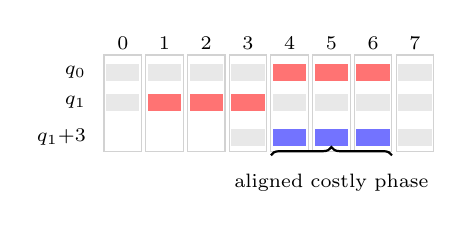
\begin{tikzpicture}[font=\scriptsize, x=5.3mm, y=5mm]
    \foreach \x in {0,...,7} {
      \node at (\x,1.75) {\x};
      \draw[gray!35] (\x-0.45,-1.0) rectangle (\x+0.45,1.45);
    }
    \node[anchor=east] at (-0.65,1) {$q_0$};
    \node[anchor=east] at (-0.65,0.25) {$q_1$};
    \foreach \x in {0,...,7} \fill[gray!18] (\x-0.4,0.78) rectangle (\x+0.4,1.22);
    \foreach \x in {0,...,7} \fill[gray!18] (\x-0.4,0.03) rectangle (\x+0.4,0.47);
    \foreach \x in {4,5,6} \fill[red!55] (\x-0.4,0.78) rectangle (\x+0.4,1.22);
    \foreach \x in {1,2,3} \fill[red!55] (\x-0.4,0.03) rectangle (\x+0.4,0.47);
    \node[anchor=east] at (-0.65,-0.65) {$q_1{+}3$};
    \foreach \x in {3,...,7} \fill[gray!18] (\x-0.4,-0.87) rectangle (\x+0.4,-0.43);
    \foreach \x in {4,5,6} \fill[blue!55] (\x-0.4,-0.87) rectangle (\x+0.4,-0.43);
    \draw[decorate, decoration={brace, amplitude=3pt}, thick]
      (3.55,-1.1) -- (6.45,-1.1) node[midway, below=3pt] {aligned costly phase};
  \end{tikzpicture}
  \caption{Why start offsets can increase sharing.  Red cells denote expensive traversal phases that do not overlap at zero offset; delaying $q_1$ by three global iterations aligns them (blue).  The offset changes time, not either query's logical levels.}
  \Description{Two query timelines have expensive phases at different global steps.  Delaying the second query shifts its expensive phase to coincide with the first.}
  \label{fig:phase-alignment}
\end{figure}


\subsection{Design Principles}

The observations lead to three principles that organize the rest of the paper.

\paragraph{P1: Share repeated neighborhood accesses exactly.}
The execution state must represent the active queries of each vertex, not only a query-oblivious union or cumulative visited set.  Exact membership lets the system read a shared neighborhood once without introducing unrelated query--edge work.

\paragraph{P2: Regularize the remaining query-state accesses.}
When broad frontiers make neighborhood sharing less selective, the engine should organize query values by graph vertex and aggregate them in a regular order.  This principle reduces effective access cost while preserving the same graph semantics.

\paragraph{P3: Schedule for realized sharing.}
Source similarity is useful only when it predicts simultaneous high-cost overlap.  The scheduler must consider relative traversal phases, batch queries with compatible overlap, and bound the delay introduced to create that overlap.

These principles explain why fusion alone is insufficient.  A global union without query membership violates P1; one fixed traversal strategy cannot satisfy both P1 and P2 across all frontier phases; and input-order batching ignores P3.  Sections~\ref{sec:overview}--\ref{sec:implementation} develop a system around these principles, while Section~\ref{sec:evaluation} assigns separate evidence to access-count reduction, access-cost reduction, and scheduling.

\section{System Overview}
\label{sec:overview}

\begin{figure*}[t]
  \centering
  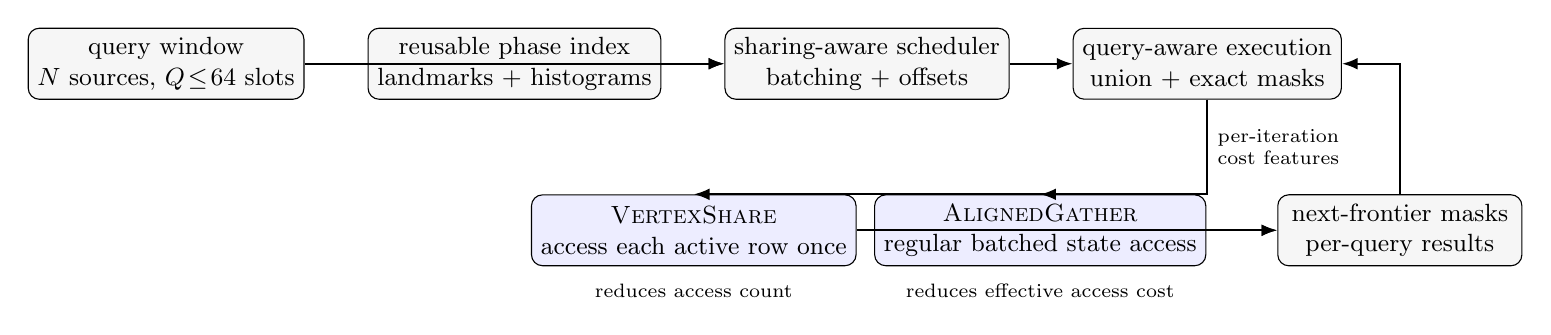
\begin{tikzpicture}[
      font=\small,
      box/.style={draw, rounded corners, minimum height=9mm, align=center, fill=gray!7},
      stage/.style={box, minimum width=31mm},
      op/.style={box, minimum width=35mm, fill=blue!7},
      arrow/.style={-{Latex[length=2mm]}, thick},
      note/.style={font=\scriptsize, align=center}
    ]
    \node[stage] (queries) {query window\\$N$ sources, $Q\!\leq\!64$ slots};
    \node[stage, right=8mm of queries] (index) {reusable phase index\\landmarks + histograms};
    \node[stage, right=8mm of index] (planner) {sharing-aware scheduler\\batching + offsets};
    \node[stage, right=8mm of planner] (state) {query-aware execution\\union + exact masks};

    \node[op, below=12mm of planner, xshift=-22mm] (push) {\sharedexpand\\access each active row once};
    \node[op, below=12mm of planner, xshift=22mm] (pull) {\coalescedgather\\regular batched state access};
    \node[stage, right=9mm of pull] (next) {next-frontier masks\\per-query results};

    \draw[arrow] (queries) -- (planner);
    \draw[arrow] (index) -- (planner);
    \draw[arrow] (planner) -- (state);
    \draw[arrow] (state.south) |- node[note, near start, right] {per-iteration\\cost features} (push.north);
    \draw[arrow] (state.south) |- (pull.north);
    \draw[arrow] (push) -- (next);
    \draw[arrow] (pull) -- (next);
    \draw[arrow] (next.north) |- (state.east);

    \node[note, below=1mm of push] {reduces access count};
    \node[note, below=1mm of pull] {reduces effective access cost};
  \end{tikzpicture}
  \caption{\system follows one memory-access objective across scheduling and execution.  The phase index exposes likely overlap, exact query masks determine what can be shared, and the runtime chooses between reducing neighborhood-access count and regularizing the remaining state access.}
  \Description{A pipeline from a query window and reusable phase index through an online scheduler and exact query-aware state to either VertexShare or AlignedGather, followed by exact next-frontier masks and query results.}
  \label{fig:overview}
\end{figure*}


\system accepts a GPU-resident graph, a set of source-based graph queries, and a resident batch limit $Q$.  Figure~\ref{fig:overview} follows the same three principles derived in Section~\ref{sec:background}.  The scheduler exposes more simultaneous overlap (P3); exact query-aware state identifies which neighborhood accesses can be shared (P1); and the execution engine chooses between vertex sharing and access-efficient aggregation for the remaining work (P2).

The phase index is built once per graph and reused across query windows.  All remaining work is query dependent.  Batching, offsets, exact frontier generation, and strategy selection count toward online cost.

\subsection{Execution Workflow}

\paragraph{1. Estimate relative traversal phases.}
The reusable index stores distances from a small set of landmarks.  For each source pair, the online scheduler constructs a histogram over relative levels.  The histogram estimates when the two queries are likely to expose common high-degree vertices.  It is an overlap hint, not an approximation of the actual frontier.

\paragraph{2. Form and align query batches.}
The scheduler places sources with compatible phase overlap into batches of at most $Q$ queries.  It improves the initial grouping with pair swaps and selects a bounded start offset for each query.  When $N>Q$, the procedure produces several independent batches that reuse the same resident workspace.

\paragraph{3. Construct exact query-aware frontiers.}
At global iteration $t$, the engine activates scheduled queries and materializes $U_t$ together with $\querymask_t$.  Current frontier, next frontier, cumulative state, and typed query values remain distinct.  Consequently, an incorrect overlap estimate may reduce sharing, but it cannot add or remove a legal query update.

\paragraph{4. Select the access strategy.}
The engine measures exact frontier size, active query--edge pairs, and neighborhood work.  It chooses \sharedexpand when current vertex overlap can remove substantial repeated topology access.  It chooses \coalescedgather when frontiers are broad and regular query-state aggregation is expected to reduce effective access cost.  The current prototype uses a threshold rule; Section~\ref{sec:selector} specifies the calibrated selector required by the final system.

\paragraph{5. Advance every query exactly.}
The selected strategy applies the algorithm's relaxation rule, records the queries whose values changed, and produces the exact union for the next iteration.  Completed queries contribute no further work.  The process terminates when every query converges and returns an ordinary per-query value vector.

Algorithm~\ref{alg:execute-batch} summarizes the workflow.  The scheduler provides only $(q,s_q,o_q)$ descriptors before execution; later decisions use exact state.  Two online costs remain explicit: feature collection and next-union construction.

\begin{algorithm}[t]
  \caption{Exact execution of one scheduled query batch}
  \label{alg:execute-batch}
  \footnotesize
  \begin{algorithmic}[1]
    \Require Graph $G$; queries $(q,s_q,o_q)$; policy $P$
    \State initialize values $X$, masks $F,N,V$, union $U\gets\emptyset$
    \State active query word $A\gets 0$; global step $t\gets 0$
    \While{some query has not converged}
      \ForAll{$q$ with start offset $o_q=t$}
        \State initialize $X[s_q,q]$; $F[s_q]\gets F[s_q]\lor 2^q$
        \State $A\gets A\lor 2^q$
      \EndFor
      \State $U\gets\Call{CompactNonzero}{F}$
      \If{$U=\emptyset$} \State $t\gets t+1$; \textbf{continue} \EndIf
      \State $z\gets\Call{MeasureExactFeatures}{G,U,F,A}$
      \State $m\gets\Call{SelectStrategy}{z,P}$; clear $N$
      \If{$m=\textsc{VertexShare}$}
        \State \Call{VertexShare}{$G,U,F,N,V,X,A,P$}
      \Else
        \State \Call{AlignedGather}{$G,N,V,X,A,P$}
      \EndIf
      \State update $A$ from changed query bits; $F\gets N$; $t\gets t+1$
    \EndWhile
    \Ensure Per-query values $X[\cdot,q]$
  \end{algorithmic}
\end{algorithm}


\subsection{Decision Scope and Semantic Authority}

\system makes decisions at three timescales (Table~\ref{tab:timescales}).  This separation lets inexpensive graph summaries guide scheduling without becoming part of the query semantics.

\begin{table}[t]
  \centering
  \caption{Decision scope and semantic authority in \system.}
  \label{tab:timescales}
  \small
  \setlength{\tabcolsep}{3pt}
  \begin{tabular}{p{0.18\columnwidth}p{0.30\columnwidth}p{0.40\columnwidth}}
    \toprule
    Time & Decision & State allowed to determine results \\
    \midrule
    graph reuse & phase index & none; summary only \\
    query batch & grouping and offsets & sources and start times only \\
    iteration & strategy and next frontier & exact masks, values, and policy \\
    \bottomrule
  \end{tabular}
\end{table}

At graph-reuse time, index error affects only later overlap scores.  At query-window time, grouping determines which queries may share resident state and offsets insert idle global iterations before a query starts.  At iteration time, the runtime may reorder legal relaxations, but it may not approximate frontier membership, cumulative state, or a policy update.

This boundary also provides safe fallbacks.  Without a phase index, \system uses input-order batches and zero offsets.  Without incoming adjacency, it uses only \sharedexpand.  If an algorithm lacks a validated phase summary, scheduling is bypassed while exact multi-query execution remains available.  Each missing component therefore removes an optimization rather than changing an answer.

\subsection{Illustrative Example}

Suppose queries $q_0$, $q_1$, and $q_3$ all contain high-degree vertex $v$ in their current frontier.  Independent execution accesses the neighbor list of $v$ three times.  \system stores $v$ once in $U_t$ and records membership mask $1011_2$.  \sharedexpand accesses the list once and applies relaxations for exactly those three queries.  Later, if the frontiers become broad, \coalescedgather visits destinations and evaluates the values of $q_0,q_1,\ldots$ for each predecessor as one regular batch.  Start offsets increase the chance of the first situation; adaptive execution determines which access strategy is appropriate for the current iteration.

\section{Design}
\label{sec:design}

This section describes \system at the graph-computation level.  It first defines the shared state that preserves query identity, then presents one strategy for reducing neighborhood-access count and another for reducing the cost of broad query-state access.  Section~\ref{sec:implementation} describes how these strategies are parallelized on a GPU.

\subsection{A Query-Aware Computation Model}

Let the active work at global iteration $t$ be
\begin{equation}
  \mathcal{A}_t=\{(v,q)\mid q\text{ is active and }v\in F_{\ell_q(t)}^q\},
  \label{eq:active-work}
\end{equation}
where $F_i^q$ is the frontier of query $q$ at its logical level $i$, and $\ell_q(t)$ maps a global iteration to that level.  Query identity is part of the work item: two queries may share a graph access, but their values and convergence conditions remain independent.  Projecting $\mathcal{A}_t$ onto vertices gives the union frontier $U_t$; the multiplicity of $v$ records how many queries can reuse its neighborhood.

Independent execution enumerates the outgoing adjacency of $v$ once for every pair $(v,q)\in\mathcal{A}_t$.  The resulting candidate work can be written as
\begin{equation}
  \mathcal{C}_t=\{(v,u,q)\mid(v,q)\in\mathcal{A}_t\land (v,u)\in E\}.
  \label{eq:candidate-work}
\end{equation}
This formulation exposes two distinct opportunities.  First, candidate generation can be factored by $v$: access the neighborhood once, then apply it to exactly the queries associated with $v$.  Second, when $\mathcal{C}_t$ is broad, the same legal candidates can be enumerated by destination and query so that accesses to query-specific state follow a regular order.  These are the logical foundations of \sharedexpand and \coalescedgather, respectively.

Scheduling operates one level earlier.  It changes the mappings $\ell_q(t)$ so queries with compatible phases contribute to the same $\mathcal{A}_t$, increasing the multiplicity of useful vertices.  It never changes the order of logical levels within a query.  Thus, scheduling controls \emph{when} reusable work appears, vertex sharing controls \emph{how often} neighborhoods are accessed, and aligned aggregation controls \emph{how} the remaining state is accessed.

Table~\ref{tab:policies} instantiates this model for the traversal policies used in the paper.  The shared work sets are independent of the value type; only candidate generation and acceptance are policy-specific.  This separation is what permits cross-query sharing without reducing the system to a BFS-only representation.

\begin{table}[t]
  \centering
  \caption{Example query policies supported by the computation model.}
  \label{tab:policies}
  \small
  \setlength{\tabcolsep}{3pt}
  \begin{tabular}{llll}
    \toprule
    Query & Value & Edge candidate & Accept \\
    \midrule
    BFS & $d_q(v)$ & $d_q(v)+1$ & first discovery \\
    SSSP & $x_q(v)$ & $x_q(v)+w(v,u)$ & smaller \\
    SSWP & $x_q(v)$ & $\min(x_q(v),w(v,u))$ & larger \\
    \bottomrule
  \end{tabular}
\end{table}

\subsection{Exact Query-Aware State}

\system stores query values in a vertex-major matrix:
\begin{equation}
  \mathrm{pos}(v,q)=v\cdot Q+q.
\end{equation}
Thus, all resident query values associated with one graph vertex form one contiguous row.  A compact active-query set disables completed or not-yet-started queries without changing the matrix shape.

Three per-vertex masks have different meanings and lifetimes.  The \emph{frontier mask} is $\querymask_t(v)$ for the current iteration.  The \emph{next-frontier mask} records queries whose values change for the next iteration.  The \emph{visited mask} is cumulative and is used by algorithms such as BFS to reject repeated discovery.  A compact vertex list contains exactly the vertices with a nonempty current frontier mask, allowing execution to enumerate $U_t$ without scanning all of $V$.

Figure~\ref{fig:state-lifecycle} shows why the masks cannot be collapsed.  Frontier membership is a per-level work predicate, visited membership is historical algorithm state, and the next mask is the result of typed updates.  Combining frontier and visited state would reprocess inactive vertices; discarding query membership would force unrelated queries to inspect every union vertex.

\begin{figure}[t]
  \centering
  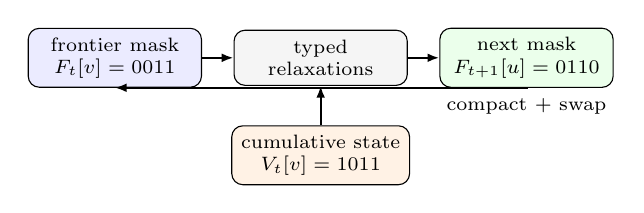
\begin{tikzpicture}[
      font=\scriptsize,
      box/.style={draw, rounded corners, align=center, minimum height=7mm, minimum width=22mm},
      arrow/.style={-{Latex[length=1.5mm]}, thick}
    ]
    \node[box, fill=blue!8] (front) {frontier mask\\$F_t[v]=0011$};
    \node[box, fill=gray!8, right=4mm of front] (op) {typed\\relaxations};
    \node[box, fill=green!8, right=4mm of op] (next) {next mask\\$F_{t+1}[u]=0110$};
    \draw[arrow] (front) -- (op);
    \draw[arrow] (op) -- (next);
    \node[box, fill=orange!10, below=5mm of op] (visited) {cumulative state\\$V_t[v]=1011$};
    \draw[arrow] (visited) -- (op);
    \draw[arrow] (next.south) |- node[below, near start] {compact + swap} (front.south);
  \end{tikzpicture}
  \caption{Masks have different meanings and lifetimes.  The current mask drives work, the cumulative mask rejects invalid rediscovery where required, and successful typed updates form the exact next mask.}
  \Description{The current frontier mask and cumulative visited mask feed typed relaxations.  Successful relaxations create a next-frontier mask, which is compacted and swapped into the next iteration.}
  \label{fig:state-lifecycle}
\end{figure}


The masks expose sharing without changing the value domain of an individual query.  For an active vertex $v$, the engine enumerates exactly the queries in $\querymask_t(v)$ and invokes their typed relaxation rule.  BFS uses first discovery, SSSP uses weighted minimum, and widest path uses bottleneck maximum.  The mask determines \emph{which queries share the vertex}; the policy determines \emph{what each query computes}.

\paragraph{Exactness invariant.}
At the start of a logical level, bit $q$ is present in $F_t[v]$ if and only if independent execution of query $q$ would process $v$ at level $\ell_q(t)$.  The compact union contains $v$ if and only if $F_t[v]$ contains at least one active query.  Parallel insertion may change the order of vertices in the compact list, but it cannot change the membership relation.  Both traversal strategies consume this invariant.

\subsection{Reducing Access Count: Vertex Sharing}
\label{sec:sharedexpand}

\sharedexpand is a source-oriented traversal over the exact union frontier.  For each $v\in U_t$, it accesses the outgoing neighbor list of $v$ once, obtains $M=\querymask_t(v)$, and applies the relaxation of each query in $M$ to every edge $(v,u)$.  Only successful query updates are inserted into the next-frontier mask of $u$.

Algorithm~\ref{alg:shared-expand} gives the logical procedure.  It separates a shared topology action---accessing the neighbor list---from query-specific value updates.  A query cannot participate merely because another query contains $v$: it must be named by the exact mask.

\begin{algorithm}[t]
  \caption{\sharedexpand: exact cross-query vertex sharing}
  \label{alg:shared-expand}
  \footnotesize
  \begin{algorithmic}[1]
    \Require CSR $G$; union $U$; masks $F,N,V$; values $X$; active $A$
    \ForAll{$v\in U$ in parallel}
      \State $M\gets F[v]\land A$
      \ForAll{$(v,u)\in G$}
        \State $S\gets 0$ \Comment{queries that improve $u$ on this edge}
        \ForAll{set bits $q$ of $M$}
          \State $c\gets P.\Call{Relax}{X[v,q],w(v,u)}$
          \If{$P.\Call{MergeUpdate}{X[u,q],c}$ succeeds}
            \State $S\gets S\lor 2^q$
          \EndIf
        \EndFor
        \If{$S\neq0$}
          \State \Call{MergeMask}{$N[u],S$}; \Call{MergeMask}{$V[u],S$}
        \EndIf
      \EndFor
    \EndFor
  \end{algorithmic}
\end{algorithm}


The neighborhood-access count is $E_{\mathrm{union}}$, compared with $E_{\mathrm{ind}}$ under independent execution.  The strategy still performs up to $E_{\mathrm{pair}}$ typed relaxations; these are necessary query work and are not counted as eliminated accesses.  Its logical work is
\begin{equation}
  O(|U_t|+E_{\mathrm{union}}+E_{\mathrm{pair}}),
\end{equation}
with $O(|V|)$ auxiliary mask and compaction state shared by the batch.  The benefit is therefore a reduction in repeated row metadata and neighbor access, not a change in the worst-case number of query-specific relaxations.

\paragraph{BFS specialization.}
Visited bits remove queries that already discovered the destination.  The remaining query bits share the same edge traversal.  This retains the principal reuse opportunity of \textsc{iBFS}~\cite{liu_ibfs_2016}, while keeping current frontier, cumulative state, and typed values separate so the computation model extends to weighted min/max traversals.

\subsection{Reducing Access Cost: Aligned Aggregation}
\label{sec:gather}

Vertex sharing is selective when frontiers are sparse and overlapping, but its destination updates become irregular as many queries and vertices are active.  \coalescedgather addresses this second regime with a destination-oriented computation.  The graph additionally stores incoming adjacency.  For a destination $v$, the strategy visits each predecessor $u$ and evaluates the resident query values
\begin{equation}
  X[u,0],X[u,1],\ldots,X[u,Q_t-1]
\end{equation}
as a contiguous group.  It reduces candidates separately for every query, compares them with $X[v,q]$, and records exactly the queries whose destination value changes.

Algorithm~\ref{alg:coalesced-gather} describes this computation without committing to a hardware mapping.  The essential choice is to hold the graph vertex fixed while varying the query identifier.  The vertex-major state layout then turns the query dimension into a regular access sequence.  The graph semantics remain the same as ordinary destination-oriented traversal; the contribution is its organization across concurrent queries.

\begin{algorithm}[t]
  \caption{\coalescedgather: access-efficient destination aggregation}
  \label{alg:coalesced-gather}
  \footnotesize
  \begin{algorithmic}[1]
    \Require Incoming CSR $G^{\mathsf T}$; masks $N,V$; values $X$; active $A$
    \ForAll{destinations $v$ in parallel}
      \ForAll{queries $q=0,\ldots,Q-1$ in vertex-major order}
        \If{$2^q\land A=0$} \State \textbf{continue} \EndIf
        \State $a_q\gets P.\mathit{identity}$
        \ForAll{$(u,v)\in G^{\mathsf T}$}
          \State $c\gets P.\Call{Relax}{X[u,q],w(u,v)}$
          \State $a_q\gets P.\Call{Reduce}{a_q,c}$
        \EndFor
        \State $b_q\gets P.\Call{Update}{X[v,q],a_q}$ ? $2^q$ : $0$
      \EndFor
      \State $M\gets b_0\lor\cdots\lor b_{Q-1}$
      \State $N[v]\gets M$; $V[v]\gets V[v]\lor M$
    \EndFor
  \end{algorithmic}
\end{algorithm}


Without early termination, \coalescedgather examines $O(Q_t|E|)$ predecessor pairs and performs $O(Q_t|V|)$ final comparisons.  It therefore does not improve the worst-case work bound and may lose badly on sparse frontiers.  It becomes attractive when frontiers are broad, many resident queries remain active, and the lower effective cost of regular state access outweighs the extra edge inspection.  This trade-off is why \coalescedgather complements rather than replaces \sharedexpand.

\subsection{Traversal Semantics and Correctness}

A query policy defines a value type, an identity or infinity value, an edge relaxation, and an order predicate for accepting an update.  BFS uses integer distance and first discovery; SSSP uses addition followed by minimum; widest path uses minimum along an edge followed by maximum at a destination.  Both strategies reuse the same query-aware state.  Dense sum algorithms such as PageRank require a separate double-buffered path and are outside the primary traversal claim.

\paragraph{Level equivalence.}
Assume a level-synchronous algorithm whose candidates are combined with an associative policy reduction.  At iteration $t$, exact $\querymask_t(v)$ contains $(v,q)$ if and only if independent query $q$ would process $v$ at logical level $\ell_q(t)$.  \sharedexpand enumerates the same outgoing edges and candidates while sharing the neighborhood access.  \coalescedgather enumerates the corresponding predecessor candidates in a different order.  The policy reduction produces the same level result, and the next mask records exactly the queries whose values change.  Induction over logical levels therefore yields the same fixed point as independent execution.

\paragraph{Why strategy switching is safe.}
Suppose the invariant holds before iteration $t$.  Both strategies evaluate the legal candidates for the same logical level and set query $q$ in the next mask exactly when $x_q(v)$ changes.  They differ only in traversal order and data-access organization.  The runtime may consequently choose a strategy independently at every level without converting query state or approximating a frontier.

\paragraph{Start offsets and termination.}
A start offset inserts inactive global iterations before a query's logical level zero; it does not alter the query's internal level sequence.  BFS terminates when it discovers no new vertex, while min/max traversals terminate when no value improves.  Terminating one query removes only its active membership; the state of other queries is unaffected.  Non-associative floating-point policies may not be bitwise reproducible, so the evaluation declares their tolerance separately.

\subsection{Sharing-Aware Query Scheduling}
\label{sec:planner}

\begin{figure}[t]
  \centering
  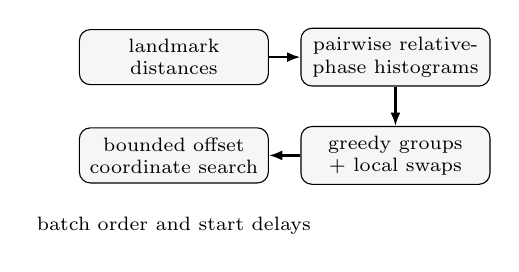
\begin{tikzpicture}[
      font=\scriptsize,
      box/.style={draw, rounded corners, align=center, minimum height=7mm, minimum width=24mm, fill=gray!7},
      arrow/.style={-{Latex[length=1.7mm]}, thick}
    ]
    \node[box] (lm) {landmark\\distances};
    \node[box, right=4mm of lm] (hist) {pairwise relative-\\phase histograms};
    \node[box, below=5mm of hist] (cluster) {greedy groups\\+ local swaps};
    \node[box, left=4mm of cluster] (offset) {bounded offset\\coordinate search};
    \draw[arrow] (lm) -- (hist);
    \draw[arrow] (hist) -- (cluster);
    \draw[arrow] (cluster) -- (offset);
    \node[below=3mm of offset, align=center] {batch order and start delays};
  \end{tikzpicture}
  \caption{The scheduler estimates relative traversal phases rather than predicting an exact execution trace.  Approximation errors remain safe because exact masks govern execution.}
  \Description{Landmark distances feed pairwise relative-phase histograms, which feed greedy grouping and local swaps, followed by a bounded coordinate search that returns batch order and start delays.}
  \label{fig:planner}
\end{figure}


The scheduler increases the input opportunity for \sharedexpand by placing compatible high-cost traversal phases in the same global iterations.  It has a reusable graph-analysis stage and a query-window stage.

\paragraph{Reusable phase index.}
The index selects up to $L=4$ landmarks using a farthest-point procedure seeded by a high-degree vertex and degree-biased samples.  A traversal from each landmark stores a 16-bit distance per vertex.  Build complexity is $O(L(|V|+|E|))$ and principal storage is approximately $2L|V|$ bytes.  Distances that exceed the representation are saturated, and unreachable vertices receive a sentinel.

For sources $s_i$ and $s_j$, landmark distances produce a histogram $H_{ij}(\delta)$ over likely overlap at relative level $\delta$.  Vertex samples are degree-weighted so that aligning a shared high-degree region scores more than aligning isolated vertices.  Pairwise histograms preserve source-pair-specific offsets that a single global source order cannot express.

\paragraph{Batch construction.}
The scheduler greedily adds the source with the largest marginal compatibility to a batch and then applies pair swaps across batches.  The batch score sums pairwise overlap under the current offsets.  Deterministic restarts reduce sensitivity to the first seed.  This is an online heuristic for a combinatorial problem; \system does not claim optimal grouping.

\paragraph{Offset selection.}
Each batch uses bounded coordinate search to select a delay in $[0,D]$ for every query; $D=16$ by default.  Each step changes one delay to maximize histogram mass at the induced pairwise offsets.  One query is anchored at zero to remove translation-equivalent schedules.  A delay penalty can account for query latency and must be calibrated on held-out workloads.

\paragraph{Fallback.}
Scheduling is bypassed when the query type lacks a meaningful phase estimator, the reusable index is unavailable, or a conservative benefit check predicts that planning cost exceeds expected access savings.  The current runner enables scheduling only for selected BFS workloads.  Existing SSSP and widest-path runs therefore establish safe execution, not cross-algorithm scheduling benefit.

Algorithm~\ref{alg:online-planner} summarizes the implemented procedure.  Batch formation uses offset-aware pair affinity, after which each batch receives bounded coordinate search.  Cross-batch swaps partially repair the fact that grouping and final offsets are not solved jointly.

\begin{algorithm}[t]
  \caption{Sharing-aware batching and bounded start-offset search}
  \label{alg:online-planner}
  \footnotesize
  \begin{algorithmic}[1]
    \Require Sources $S$; phase index $I$; batch size $Q$; delay bound $D$
    \ForAll{source pairs $(s_i,s_j)$}
      \State build weighted relative-level scores $H_{ij}[-D{:}D]$
      \State affinity $W_{ij}\gets\max_{\delta}H_{ij}(\delta)$
    \EndFor
    \While{an unassigned source remains}
      \State seed a batch with maximum remaining total affinity
      \State greedily add the source with maximum marginal $W$ score
    \EndWhile
    \Repeat
      \State apply the positive-gain cross-batch swap with largest gain
    \Until{no positive swap exists or the swap budget is exhausted}
    \ForAll{batches $B$}
      \State initialize offsets from zero, completion alignment, and six seeds
      \ForAll{initial offset vectors $o$}
        \Repeat
          \ForAll{$q\in B$} \State choose $o_q\in[0,D]$ maximizing pair score \EndFor
        \Until{a pass makes no change or eight passes finish}
      \EndFor
      \State retain the highest-score normalized offset vector
    \EndFor
    \Ensure Ordered batches and per-query start offsets
  \end{algorithmic}
\end{algorithm}


\subsection{Adaptive Strategy Selection}
\label{sec:selector}

The desired selector estimates the memory-related cost of both strategies from exact counters already produced by execution:
\begin{align}
 C_{\mathrm{VS}} &= a_0 + a_1 E_{\mathrm{union}}
                    +a_2 E_{\mathrm{pair}}+a_3 A_t, \\
 C_{\mathrm{AG}} &= b_0 + b_1 E_{\mathrm{in}}
                    +b_2 R_{\mathrm{state}}(Q_t)+b_3 |V|,
\end{align}
where $A_t$ counts active destination--query pairs, $E_{\mathrm{in}}$ is incoming edge inspection, and $R_{\mathrm{state}}$ estimates the cost of regular batched state access.  Coefficients may depend on deployment hardware and value width, but should transfer across graphs on the same platform.  Hysteresis prevents unstable switching near the crossover.

Figure~\ref{fig:selector-space} shows the qualitative boundary.  High exact overlap favors \sharedexpand; broad frontiers and high query activity amortize the fixed inspection cost of \coalescedgather.  The boundary is deliberately conceptual because its measured position depends on graph structure, value width, and platform.

\begin{figure}[t]
  \centering
  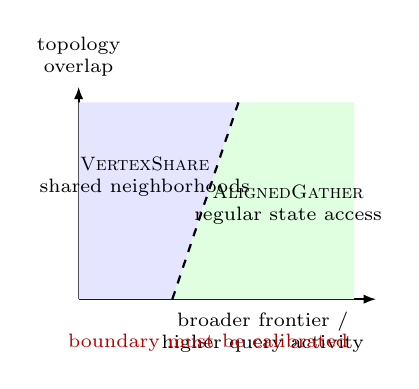
\begin{tikzpicture}[font=\scriptsize, x=3.5cm, y=2.5cm]
    \draw[-{Latex[length=1.6mm]}, thick] (0,0) -- (1.08,0)
      node[below left=1pt, align=center] {broader frontier /\\higher query activity};
    \draw[-{Latex[length=1.6mm]}, thick] (0,0) -- (0,1.08)
      node[above, align=center] {topology\\overlap};
    \fill[blue!10] (0,0) -- (0,1) -- (0.58,1) -- (0.34,0) -- cycle;
    \fill[green!12] (0.34,0) -- (0.58,1) -- (1,1) -- (1,0) -- cycle;
    \draw[dashed, thick] (0.34,0) -- (0.58,1);
    \node[align=center] at (0.24,0.62) {\sharedexpand\\shared neighborhoods};
    \node[align=center] at (0.76,0.48) {\coalescedgather\\regular state access};
    \node[align=center, text=red!70!black] at (0.47,-0.22)
      {boundary must be calibrated};
  \end{tikzpicture}
  \caption{Conceptual strategy space, not a measured decision boundary.  Exact topology overlap favors \sharedexpand; broad frontiers and high query activity favor \coalescedgather.  The final selector must learn the crossover on held-out workloads.}
  \Description{A conceptual two-dimensional space has topology overlap on the vertical axis and frontier breadth or query activity on the horizontal axis. A dashed boundary separates VertexShare and AlignedGather regions.}
  \label{fig:selector-space}
\end{figure}


\paragraph{Current implementation.}
The checked-in selector does not yet implement this calibrated model.  It chooses \coalescedgather when
\begin{equation}
 E_{\mathrm{virtual}} \geq \tau Q_t|E|,
\end{equation}
with default $\tau=0.20$; BFS remains in that strategy after switching.  $E_{\mathrm{virtual}}$ counts query-weighted expansion work.  The threshold is interpretable but does not separately model neighborhood-access savings and regular state-access cost.  \drafttodo{Fit the two-strategy model on a disjoint training subset; freeze coefficients; compare it with the threshold, fixed strategies, and a per-iteration oracle on held-out graph/query pairs.}

\subsection{Alternatives Considered}

\paragraph{Independent query execution.}
It preserves per-query simplicity but does not remove repeated neighborhood access or organize state across queries.  It remains an essential baseline.

\paragraph{One global union without exact membership.}
It accesses a neighborhood once but evaluates every query for every union vertex, replacing repeated topology access with false query--edge work.  Exact masks avoid this failure mode.

\paragraph{One fixed traversal strategy.}
Always using vertex sharing is inefficient for broad phases with irregular destination state access; always using aligned aggregation examines too much topology for sparse phases.  A selector is necessary only if its saved cost exceeds measurement and switching overhead.

\paragraph{Single scalar source order.}
Sorting sources by distance to one landmark is inexpensive but cannot express pair-specific relative phases.  It is included as a \textsc{Glign}-compatible ablation rather than treated as sufficient scheduling.

\paragraph{Immediate query replenishment.}
Reusing a resident slot as soon as a query completes can increase occupancy, but current measurements show that mixing traversal phases often increases total access work.  \system therefore executes a closed, phase-aligned batch by default.

\begin{table*}[t]
  \centering
  \caption{Logical design choices and the evidence required to justify them.}
  \label{tab:design-alternatives}
  \small
  \begin{tabular}{p{0.20\textwidth}p{0.20\textwidth}p{0.27\textwidth}p{0.23\textwidth}}
    \toprule
    Decision & \system choice & Alternative and trade-off & Required evidence \\
    \midrule
    query-aware state & exact level mask + typed value & query-oblivious union adds false work; BFS-only bits restrict algorithms & query--edge work and multi-algorithm correctness \\
    access-count reduction & one traversal per union vertex & per-query execution repeatedly accesses shared neighborhoods & neighborhood bytes at fixed query--edge work \\
    access-cost reduction & vertex-major batched aggregation & independent query order produces irregular state access & requests and exposed stalls per useful value \\
    temporal coordination & pairwise phases + bounded offsets & scalar source order misses pair-specific alignment & predicted versus realized overlap over many seeds \\
    adaptive execution & exact counters + calibrated model & one fixed mode is simpler but phase-sensitive & held-out regret against a strategy oracle \\
    \bottomrule
  \end{tabular}
\end{table*}

\section{Implementation}
\label{sec:implementation}

We implement \system as a header-only C++17/CUDA library with 7,574 lines in public and internal headers.  CMake selects CUDA architecture 7.5 by default, and preliminary measurements use release builds.  Access traits abstract graph storage, compile-time policies define algorithm behavior, and runtime descriptors provide query sources and parameters.

\paragraph{Graph and query state.}
The source-oriented strategy reads outgoing CSR.  The destination-oriented strategy also reads incoming CSR.  Weighted algorithms use an aligned edge-weight array.  One engine workspace owns the vertex-major value matrix; current, next, and cumulative query masks; compact union frontiers; scan offsets; access counters; and the active-query set.  When $N>Q$, batches reuse this workspace, so memory scales with resident queries rather than window size.

For a $w$-byte value, the value matrix requires $w|V|Q$ bytes.  Three 64-bit masks add $24|V|$ bytes, independent of $Q$ up to 64.  Compact lists, flags, and scan offsets add $O(|V|)$ storage.  Table~\ref{tab:workspace} summarizes the principal structures; graph CSR and its transpose are reported separately in the evaluation.

\begin{table}[t]
  \centering
  \caption{Principal device structures, excluding graph CSR and its transpose.}
  \label{tab:workspace}
  \small
  \begin{tabular}{lll}
    \toprule
    Structure & Approx. bytes & Lifetime \\
    \midrule
    typed values & $w|V|Q$ & batch \\
    three query masks & $24|V|$ & batch \\
    union vertex lists & $2s_v|V|$ & batch \\
    scan/flag arrays & $O(|V|)$ & batch \\
    phase distances & $2L|V|$ & graph reuse \\
    counters/active word & $O(1)$ & iteration \\
    \bottomrule
  \end{tabular}
\end{table}

\paragraph{GPU mapping.}
This paragraph contains the hardware-specific mapping deliberately omitted from the conceptual design.  \sharedexpand assigns one active union vertex to a cooperative execution group; the current default uses a warp for a vertex and distributes high- and low-degree rows across blocks for load balance.  \coalescedgather maps the query identifier to the contiguous dimension of a CUDA block while holding a destination row fixed.  As Figure~\ref{fig:layout} shows, this mapping follows the vertex-major state layout and turns one vertex's query values into consecutive accesses.

\begin{figure}[t]
  \centering
  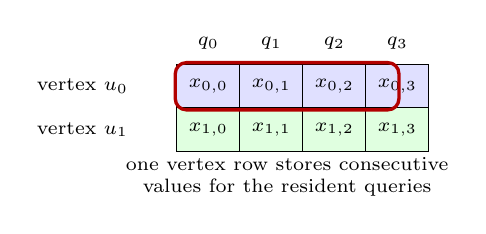
\begin{tikzpicture}[
      font=\scriptsize,
      cell/.style={draw, minimum width=8mm, minimum height=5.5mm, inner sep=0pt},
      lab/.style={align=right}
    ]
    \node[lab] at (-1.2,0) {vertex $u_0$};
    \node[lab] at (-1.2,-0.55) {vertex $u_1$};
    \foreach \x/\q in {0/0,1/1,2/2,3/3} {
      \node at (0.4+0.8*\x,0.55) {$q_{\q}$};
      \node[cell, fill=blue!12] at (0.4+0.8*\x,0) {$x_{0,\q}$};
      \node[cell, fill=green!12] at (0.4+0.8*\x,-0.55) {$x_{1,\q}$};
    }
    \draw[very thick, red!70!black, rounded corners] (-0.02,-0.3) rectangle (2.82,0.3);
    \node[align=center] at (1.4,-1.15) {one vertex row stores consecutive\\values for the resident queries};
  \end{tikzpicture}
  \caption{Vertex-major $V\!\times\!Q$ state layout used by \coalescedgather.  Holding the graph vertex fixed while varying the query identifier turns the query dimension into a contiguous access sequence.}
  \Description{A two-row value matrix with vertices as rows and resident queries as contiguous columns. A highlighted row contains all query values for one graph vertex.}
  \label{fig:layout}
\end{figure}


\paragraph{Frontier construction.}
Atomic updates merge successful query bits at a destination.  A first-writer test records whether the destination needs a compact-list entry; a prefix scan then produces the next union frontier and counts unique vertices and query--edge pairs.  Both traversal strategies emit the same compact format.  These operations are included in end-to-end time because omitting them would overstate the benefit of sharing.

\paragraph{Execution variants.}
The implementation retains vertex-parallel, query-parallel, and shared-vertex expansion kernels for controlled comparison.  The aligned path has a direct row--query kernel and a neighbor-tiled shared-memory variant.  The direct kernel uses 128 CUDA threads: it processes two destination rows at $Q=64$ and four at $Q=32$.  Current focused experiments find that synchronization and shared-memory traffic outweigh neighbor-identifier reuse in the tiled variant, so the direct path is the default.  These variants are implementation alternatives, not separate paper contributions.

\paragraph{Scheduled activation.}
Per-query start levels are stored in a host-generated schedule and converted to an activation mask at each global step.  Activating a query initializes only its source value and source frontier bit.  Inactive queries are filtered in both strategies, so offsets require neither clearing nor reallocating the $V\!\times\!Q$ matrix.

\paragraph{Strategy selection.}
Before a hybrid decision, a GPU kernel sums union edges, query-weighted edges, and active pairs into 64-bit counters.  The current engine copies them to the host before launching the selected strategy.  This path is useful for instrumentation but introduces per-iteration synchronization.  The final implementation should compare host selection with a device-side decision or a CUDA Graph path; all end-to-end measurements include the current control cost.

\paragraph{Phase-index persistence.}
The reusable index stores graph dimensions, landmark identifiers and weights, and landmark-major 16-bit distances.  Build and load are separate code paths.  The online runner loads an existing index when available and charges query-dependent evaluation to the window, while reporting build time, load time, size, and break-even windows separately.

\paragraph{Measurement and correctness.}
The runner executes input-order, batch-only, offset-only, and full schedules through the same engine.  It reports GPU execution time, scheduling time, union and query-weighted edge counts, and result fingerprints.  Focused profiling uses NVIDIA Nsight Compute; complete runs use CUDA events and host timers.  Debug tests compare all output values, while experiment runs additionally store per-query fingerprints.  The runtime rejects batches above 64 queries, invalid sources, unsupported schedules, and aligned aggregation without incoming adjacency.

\paragraph{Current engineering boundary.}
The prototype contains exact query masks, typed BFS/SSSP/widest-path policies, both traversal strategies, the phase index, grouping and offset search, and the threshold selector.  It does not yet contain the calibrated model in Section~\ref{sec:selector}.  A final claim about adaptive strategy selection is contingent on implementing and evaluating that model.

\section{Evaluation}
\label{sec:evaluation}

The evaluation tests whether the memory-access view yields an effective CGQ system.  It separates three mechanisms from end-to-end performance: neighborhood sharing, regular state access, and scheduling-induced reuse.  Blue text denotes reproducible but preliminary measurements from the current repository; red text marks experiments still required before submission.

We organize the section around six questions:
\begin{description}
  \item[RQ1: Overall performance.] Does one fixed \system configuration improve query-window throughput and latency over strong graph-system and CGQ baselines?
  \item[RQ2: Memory behavior.] Do fewer neighborhood accesses and lower state-access stalls explain performance?
  \item[RQ3: Component effectiveness.] What does vertex sharing, aligned aggregation, adaptive selection, and scheduling contribute individually?
  \item[RQ4: Scheduling quality.] Do grouping and offsets increase realized vertex sharing after online cost and query delay?
  \item[RQ5: Generality and scaling.] Do the benefits persist across graph structure, query count, batch size, algorithms, and devices?
  \item[RQ6: Overhead and correctness.] What preprocessing, online, memory, and semantic costs does \system introduce?
\end{description}

\subsection{Experimental Setup}

\paragraph{Platform.}
Existing measurements use one NVIDIA Tesla V100-SXM2 with 32~GiB HBM2, CUDA 12.8, and release compilation.  Unless stated otherwise, query sources are distinct, reusable index construction is excluded, online scheduling is included, and correctness is checked against per-query fingerprints.  The online runner uses two warmups, five measured repetitions, alternating method order, and reports the median.  Final experiments will add a recent GPU generation and at least seven measured repetitions with confidence intervals.

\paragraph{Datasets.}
Table~\ref{tab:datasets} spans citation, web, and social graphs with different degree distributions.  The final suite should add a long-diameter road graph and a synthetic family with controlled degree skew and source overlap.  Directed inputs retain their directions; \coalescedgather materializes incoming adjacency.

\begin{table}[t]
  \centering
  \caption{Graphs in existing experiments.  B and M denote billions and millions.}
  \label{tab:datasets}
  \small
  \begin{tabular}{lrr}
    \toprule
    Graph & $|V|$ & $|E|$ \\
    \midrule
    cit-Patents & 3.77M & 33.04M \\
    soc-Orkut & 3.00M & 212.70M \\
    soc-LiveJournal1 & 4.85M & 137.99M \\
    indochina-2004 & 7.41M & 304.47M \\
    soc-Twitter & 21.30M & 530.05M \\
    soc-SinaWeibo & 58.66M & 522.64M \\
    \bottomrule
  \end{tabular}
\end{table}

\paragraph{Queries.}
We evaluate BFS, SSSP with nonnegative weights, and single-source widest path (SSWP).  Main experiments use $N=256,Q=64$ and sweep $N\in\{64,128,256,512,1024\}$ and $Q\in\{1,2,4,8,16,32,64\}$.  Query latency begins at window admission, so scheduling delay remains visible.  Uniform distinct sources are the reproducible default; high-degree-biased, community-local, and adversarial low-overlap sources exercise different sharing regimes.  Every family uses at least ten stored source vectors.

\paragraph{Baselines.}
The main comparison includes: independent execution in the same engine; independent concurrent execution; Gunrock~\cite{wang_gunrock_2016} and TGraph~\cite{zhang_tgraph_2025} where their artifacts support the same graph and algorithm; \textsc{iBFS} for BFS~\cite{liu_ibfs_2016}; and a \textsc{Glign}-compatible grouping and delay policy on \system's execution engine~\cite{yin_glign_2022}.  The same-engine baselines isolate CGQ mechanisms from language and implementation differences.  CGgraph and CompressGraph address out-of-memory and compressed single-query execution, respectively, so they provide design context rather than a universal speedup denominator.

\paragraph{Metrics and fairness.}
Window throughput is $N/T_{\mathrm{wall}}$ and includes query-dependent scheduling.  We report absolute time, queries/s, P50/P95 query latency, peak memory, and out-of-memory outcomes.  Access metrics include $E_{\mathrm{ind}}$, $E_{\mathrm{union}}$, $E_{\mathrm{pair}}$, device memory bytes, requests per useful value, and exposed data-access stalls.  Every main result uses one frozen policy rather than the best configuration selected separately for each graph.  Systems receive the same orientation, weights, sources, semantics, memory limit, warmups, and repetitions.  \drafttodo{Rerun all systems from one clean commit on an exclusive machine and publish source vectors, raw repetitions, checksums, clocks, and commands.}

\subsection{RQ1: Overall CGQ Performance}

\paragraph{Hypothesis.}
If access savings exceed mask maintenance, frontier construction, and scheduling cost, one fixed \system configuration should improve query-window throughput without hiding delay in its constituent queries.  The primary result will report queries/s and absolute time over all graph--algorithm pairs, normalized to the strongest applicable baseline, with a separate common-capacity comparison for systems that cannot hold $Q=64$.

\drafttodo{Produce the fixed-policy $N=256,Q=64$ main table after implementing and freezing the selector.  Include independent execution, Gunrock/TGraph where applicable, iBFS, the Glign-compatible schedule, GraphWeft, scheduling time, total time, queries/s, P50/P95 latency, and peak device memory.}

The current external result is not yet a positive end-to-end claim.  Table~\ref{tab:ibfs-gap} compares the fixed online-hybrid BFS path with \textsc{iBFS} at $N=256,Q=64$.  \preliminary{Its geometric-mean speedup is only $0.49\times$.}  This result shows that the current combination of sharing and scheduling does not compensate for the maturity and BFS specialization of \textsc{iBFS} at this batch size.

\begin{table}[t]
  \centering
  \caption{Preliminary fixed-$Q=64$ BFS comparison.  Speedup is iBFS time divided by \system time; higher favors \system.}
  \label{tab:ibfs-gap}
  \small
  \begin{tabular}{lrrr}
    \toprule
    Graph & \system (ms) & iBFS (ms) & Speedup \\
    \midrule
    cit-Patents & 967.87 & 298.36 & 0.31$\times$ \\
    soc-Orkut & 1679.54 & 1030.02 & 0.61$\times$ \\
    soc-Twitter & 10268.30 & 3463.27 & 0.34$\times$ \\
    soc-SinaWeibo & 5704.68 & 5180.71 & 0.91$\times$ \\
    \midrule
    Geometric mean & --- & --- & 0.49$\times$ \\
    \bottomrule
  \end{tabular}
\end{table}

Two follow-ups gate the final claim.  First, the batch-size sweep must reproduce on the current code the earlier observation that \system is more competitive at $Q=16$ and $Q=32$.  Second, the same engine must compare an iBFS-like bitwise BFS, a \textsc{Glign}-compatible schedule, their combination, and the full \system.  This decomposition distinguishes a general memory-access design from a composition of prior BFS and scheduling techniques.

\paragraph{Current conclusion.}
The current $Q=64$ evidence rejects end-to-end superiority for BFS.  It narrows the immediate task to locating the batch-size crossover, removing hybrid regressions, and testing whether typed multi-algorithm execution adds value after controlling for an iBFS-like specialization.

\subsection{RQ2: Memory-Access Behavior}

\paragraph{Hypothesis.}
\sharedexpand should improve time only when it reduces realized neighborhood access, while \coalescedgather should improve time only when regular state access reduces memory requests or exposed stalls enough to offset additional edge inspection.  We test two causal chains:
\[
 \text{sharing}\rightarrow E_{\mathrm{union}}/E_{\mathrm{ind}}
 \rightarrow\text{topology bytes}\rightarrow\text{time},
\]
\[
 \text{aggregation}\rightarrow\text{requests/value}
 \rightarrow\text{access stalls}\rightarrow\text{time}.
\]
The controlled comparison holds the logical query--edge pairs and output values fixed while changing data organization and traversal order.

Existing profiles support the bottleneck diagnosis but not yet the full causal chain.  In one representative $Q=32$ aggregation iteration per graph, achieved bandwidth is 31--62\% of peak while long-latency dependency stalls account for 43--60\% (Table~\ref{tab:ncu}).  Sampling one iteration cannot characterize a complete query window.

\begin{table}[t]
  \centering
  \caption{Preliminary profile of one $Q=32$ aggregation iteration per graph.}
  \label{tab:ncu}
  \small
  \begin{tabular}{lrrr}
    \toprule
    Graph & GB/s & Peak BW & Access stall \\
    \midrule
    cit-Patents & 531.8 & 59.2\% & 59.8\% \\
    soc-Orkut & 557.3 & 62.0\% & 46.5\% \\
    soc-Twitter & 278.4 & 31.0\% & 51.7\% \\
    soc-SinaWeibo & 472.9 & 52.6\% & 43.1\% \\
    \bottomrule
  \end{tabular}
\end{table}

\drafttodo{Collect stratified or full-run profiles; compare vertex-major and query-major state, plus direct and alternative aggregation, for 4-, 8-, and 16-byte values.}

\paragraph{Current conclusion.}
The samples establish that exposed data-access latency is significant in the target workload, but they do not yet prove that \coalescedgather reduces it relative to a controlled alternative.  That proof requires identical logical work, values, and frontier inputs.

\subsection{RQ3: Component Effectiveness}

\paragraph{Hypothesis.}
Each component should move the memory quantity it targets: query-aware masks should eliminate false query--edge work, \sharedexpand should reduce neighborhood accesses, \coalescedgather should reduce effective state-access cost in broad phases, and the selector should approach the faster strategy without per-graph tuning.

The ablation compares independent execution; a query-oblivious union; exact masks with fixed \sharedexpand; exact masks with fixed \coalescedgather; the existing threshold; the calibrated selector; and a measured per-iteration oracle.  Controlled frontier replays vary union size, mask population, degree, active query count, and value width independently.  Whole-query runs then test whether the learned crossover transfers to natural frontier sequences.  Selector quality is reported as regret relative to the oracle, switching frequency, and measurement/model overhead.

\drafttodo{Implement the model in Section~\ref{sec:selector}, create graph-disjoint calibration and test splits, and explain the current Twitter hybrid regression.}

\subsection{RQ4: Sharing-Aware Scheduling}

\paragraph{Hypothesis.}
If the phase estimator captures useful overlap, higher schedule scores should produce lower $E_{\mathrm{union}}/E_{\mathrm{ind}}$ after online cost, without unacceptable query delay.  Table~\ref{tab:planner-prelim} reports the strongest current mechanism result: all-push BFS, $N=128,Q=32$, seed 42, comparing online grouping plus offsets with input-order batches at zero offset.  \preliminary{Speedups range from $1.15\times$ to $2.31\times$, and the largest gains coincide with the largest reductions in union-edge access.}

Figure~\ref{fig:planner-result} places the execution benefit beside the remaining neighborhood work.  The trend is consistent with the access-count hypothesis, but the single seed, BFS-only workload, and per-graph landmark configurations do not establish general scheduling quality.

\begin{figure*}[t]
  \centering
  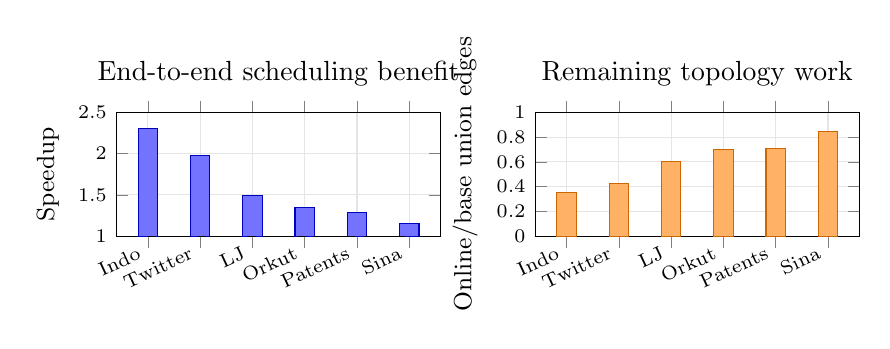
\begin{tikzpicture}
    \begin{groupplot}[
        group style={group size=2 by 1, horizontal sep=1.2cm},
        width=0.47\textwidth,
        height=0.26\textwidth,
        ybar,
        /pgf/bar width=7pt,
        symbolic x coords={Indo,Twitter,LJ,Orkut,Patents,Sina},
        xtick=data,
        x tick label style={rotate=25,anchor=east,font=\scriptsize},
        tick label style={font=\scriptsize},
        label style={font=\small},
        grid=major,
        grid style={gray!20},
        enlarge x limits=0.12
      ]
      \nextgroupplot[ymin=1,ymax=2.5,ylabel={Speedup},
                     title={End-to-end scheduling benefit}]
        \addplot[fill=blue!55,draw=blue!75!black]
          coordinates {(Indo,2.309) (Twitter,1.983) (LJ,1.489)
                       (Orkut,1.342) (Patents,1.290) (Sina,1.152)};
        \draw[dashed,black] (axis cs:Indo,1) -- (axis cs:Sina,1);
      \nextgroupplot[ymin=0,ymax=1,ylabel={Online/base union edges},
                     title={Remaining topology work}]
        \addplot[fill=orange!60,draw=orange!80!black]
          coordinates {(Indo,0.356) (Twitter,0.428) (LJ,0.601)
                       (Orkut,0.698) (Patents,0.707) (Sina,0.845)};
        \draw[dashed,black] (axis cs:Indo,1) -- (axis cs:Sina,1);
    \end{groupplot}
  \end{tikzpicture}
  \caption{Existing all-push BFS result for $N=128,Q=32$ and seed 42.  Online grouping and offsets improve end-to-end time by $1.15\times$--$2.31\times$ (left); the largest gains coincide with the largest reductions in union-edge work (right).  Scheduling time is included and index construction is excluded.}
  \Description{Two bar charts for six graphs. The left chart shows scheduling speedups from 1.15 to 2.31. The right chart shows the remaining union-edge ratios from 0.356 to 0.845, with lower ratios generally corresponding to higher speedups.}
  \label{fig:planner-result}
\end{figure*}


\begin{table*}[t]
  \centering
  \caption{Preliminary online scheduling result: all-push BFS, $N=128,Q=32$.  Baseline is input-order batching with zero offsets; scheduling time is included.}
  \label{tab:planner-prelim}
  \small
  \begin{tabular}{lrrrrrr}
    \toprule
    Graph & Baseline (ms) & Scheduled (ms) & Speedup & Sched. (ms) & Baseline union edges & Scheduled union edges \\
    \midrule
    indochina-2004 & 1116.43 & 483.42 & 2.31$\times$ & 10.69 & 9.278B & 3.302B \\
    soc-Twitter & 5160.31 & 2602.48 & 1.98$\times$ & 11.87 & 9.462B & 4.054B \\
    soc-LiveJournal1 & 1032.91 & 693.50 & 1.49$\times$ & 13.14 & 2.367B & 1.422B \\
    soc-Orkut & 1459.51 & 1087.66 & 1.34$\times$ & 14.49 & 2.887B & 2.016B \\
    cit-Patents & 1039.62 & 806.09 & 1.29$\times$ & 14.20 & 0.745B & 0.527B \\
    soc-SinaWeibo & 5571.70 & 4834.70 & 1.15$\times$ & 11.24 & 4.973B & 4.202B \\
    \bottomrule
  \end{tabular}
\end{table*}

The six-graph ordering is monotonic: indochina retains 35.6\% of baseline union-edge work and has the largest speedup, while SinaWeibo retains 84.5\% and has the smallest.  Online scheduling takes 10.7--14.5~ms and is included in the scheduled time.  This small sample supports the proposed mechanism but is not a general correlation result.

The newer $N=256,Q=64$ runner adds a conservative automatic gate (Table~\ref{tab:planner-gating}).  It enables full scheduling for cit-Patents and Twitter and uses the fallback for the other two cases.  The gate avoids regressions in the tested neutral cases, but the four-graph geometric-mean benefit is only $1.064\times$.

\begin{table}[t]
  \centering
  \caption{Preliminary automatic scheduling for BFS at $N=256,Q=64$.  Online evaluation is included; disabled rows use the fallback.}
  \label{tab:planner-gating}
  \small
  \begin{tabular}{lrrr}
    \toprule
    Graph & Schedule & Speedup & Eval. ms \\
    \midrule
    cit-Patents & full & 1.148$\times$ & 26.62 \\
    soc-Orkut & disabled & 1.000$\times$ & 0.02 \\
    soc-Twitter & full & 1.119$\times$ & 15.10 \\
    soc-SinaWeibo & disabled & 1.000$\times$ & 0.11 \\
    \midrule
    Geometric mean & auto & 1.064$\times$ & --- \\
    \bottomrule
  \end{tabular}
\end{table}

The final ablation compares input order, random order, degree grouping, a scalar-landmark \textsc{Glign}-compatible policy, pairwise histograms, pair swaps, zero offsets, completion-aligned offsets, and bounded coordinate search.  It reports predicted score, realized $S_{\mathrm{share}}$, execution and scheduling time, and P50/P95 latency over at least ten source sets, including low-overlap adversarial queries.

\paragraph{Current conclusion.}
For this all-push BFS sample, lower realized neighborhood access accompanies higher speedup, and a simple gate avoids the tested neutral Q64 cases.  Existing data does not yet establish multi-seed robustness, incremental value over \textsc{Glign}, or scheduling benefit for weighted traversals.

\subsection{RQ5: Generality and Scaling}

\paragraph{Hypothesis.}
Sharing should initially improve with $Q$ as more overlap becomes available, then flatten or reverse when resident state and query--edge work dominate.  The $N$ sweep separates resident batch size from total window throughput.  Source sets are stratified by predicted and realized overlap; synthetic graphs vary average degree, skew, diameter, and community structure.

Cross-device experiments use the V100 and one recent GPU with a different memory/compute balance.  Selector coefficients may be calibrated once per device, not per graph.  Weighted algorithms use several weight distributions and verify that a BFS phase index is not credited for behavior it cannot predict.  \drafttodo{Design SSSP- and SSWP-appropriate phase summaries, or narrow the scheduling claim to BFS while retaining the general execution model.}

\subsection{RQ6: Overhead and Correctness}

Reusable index and resident state should amortize across repeated query windows before erasing execution savings.  We report memory for CSR, transpose, weights, value matrix, masks, compaction workspace, and phase index.  Online cost is decomposed into index load, histogram construction, grouping, swaps, offset search, exact counters, and union construction.  Break-even analysis finds the minimum sharing level and number of windows required to recover each cost.

The current serial CPU index builder takes about 30.3~s/0.88~GiB for indochina, 45.8~s/0.58~GiB for LiveJournal, and 116.7~s/1.27~GiB for Twitter.  These costs must be reported rather than treated as free preprocessing.

Correctness compares every query result with independent execution.  Existing validation covers 60 real-graph runs and 27 small-graph combinations across BFS/SSSP/SSWP, $Q\in\{1,32,64\}$, and both fixed and hybrid strategies.  The final artifact adds randomized graphs, disconnected components, duplicate sources, unreachable vertices, large distances, weighted ties, saturated landmark distances, $N$ not divisible by $Q$, and maximum offset.  Integral outputs use exact equality; floating-point policies declare tolerance and determinism limits.

\subsection{Evidence Summary}

Current evidence establishes three narrower facts: scheduled exact execution is correct on the tested cases; phase alignment can substantially reduce neighborhood accesses for selected BFS windows; and exposed data-access latency is significant in the sampled aggregation phases.  It does \emph{not} yet establish that a frozen \system configuration beats \textsc{iBFS}, that aligned aggregation causes lower access cost, that the selector transfers across graphs, or that scheduling benefits weighted algorithms.  These are the gating experiments for a defensible SIGMOD/VLDB claim.

\FloatBarrier
\section{Related Work}
\label{sec:related}

\begin{table*}[t]
  \centering
  \caption{Positioning against representative database and concurrent graph systems.  The systems optimize different sources of graph-processing cost; entries describe scope rather than performance.}
  \label{tab:positioning}
  \small
  \setlength{\tabcolsep}{4pt}
  \begin{tabular}{p{0.09\textwidth}p{0.15\textwidth}p{0.22\textwidth}p{0.25\textwidth}p{0.18\textwidth}}
    \toprule
    System & Workload & Reuse or bottleneck & Main approach & Algorithm/platform scope \\
    \midrule
    TGraph & one analytic & accelerator portability & tensor-centric model and tensor graph operations & multiple analytics, multiple accelerators \\
    CGgraph & one analytic & cross-iteration graph reuse and limited device memory & retain reusable subgraph; cooperative processing & multiple analytics, CPU--GPU \\
    Compress\-Graph & one analytic & repeated neighbor sequences & rule-based compression and direct execution & multiple analytics, CPU/GPU \\
    iBFS & concurrent BFS & cross-query frontier overlap & shared BFS state and direction selection & BFS, GPU \\
    Glign & concurrent traversals & temporal phase misalignment & landmark affinity, grouping, and delayed starts & iterative traversals \\
    \system & concurrent queries & repeated neighborhoods and irregular query-state access & exact vertex sharing, aligned aggregation, and phase scheduling & BFS/SSSP/SSWP, GPU \\
    \bottomrule
  \end{tabular}
\end{table*}

\paragraph{Database graph analytics systems.}
Recent SIGMOD/VLDB systems begin from a graph-processing limitation and introduce a computation model before hardware optimization.  TGraph uses tensor computation runtimes to provide one graph model across accelerator backends and adds tensor-based compression and out-of-memory processing~\cite{zhang_tgraph_2025}.  CGgraph addresses limited GPU memory and CPU--GPU imbalance by retaining a reusable subgraph and allocating tasks on demand~\cite{cui_cggraph_2024}.  CompressGraph represents repeated neighbor sequences as rules and reuses intermediate results while executing directly on the compressed graph~\cite{chen_compressgraph_2023}.  Gunrock provides a programmable frontier abstraction and efficient single-query GPU graph execution~\cite{wang_gunrock_2016}, while direction-optimizing BFS reduces examined edges by changing traversal direction~\cite{beamer_direction_2013}.  These systems motivate our abstraction-first presentation and strong single-query baselines.  Their primary workload is one analytic, whereas \system studies reuse and access organization across a window of independent queries.

\paragraph{Concurrent BFS and traversal alignment.}
\textsc{iBFS} jointly executes multiple BFS instances with shared frontier and status state and supports both traversal directions~\cite{liu_ibfs_2016}.  It is the closest BFS baseline and already demonstrates cross-query neighborhood reuse.  \system retains exact current-query membership separately from cumulative state, supports typed min/max policies, and connects sharing with phase scheduling and broad state aggregation.  These differences require a same-engine decomposition rather than a claim based only on external runtimes.

\textsc{Glign} observes that queries reach expensive graph regions at different times and uses high-degree landmarks, affinity grouping, and delayed starts~\cite{yin_glign_2022}.  \system adopts temporal alignment but estimates pair-specific relative phases and optimizes realized neighborhood access.  More importantly, scheduling is one component of a memory-access design that also determines how shared and non-shared state is executed.  A \textsc{Glign}-compatible policy on the same engine isolates this incremental value.

\paragraph{General concurrent graph processing.}
MITra formalizes multi-instance traversal and synthesizes shared algorithms from ranks and edge functions~\cite{li_mitra_2023}; AutoMI automates vectorized distributed graph computation~\cite{zhao_automating_2024}; and Krill uses compiler and runtime support for concurrent graph processing~\cite{chen_krill_2021}.  Seraph separates graph structure, runtime state, and computation so cluster jobs can share graph resources~\cite{xue_seraph_2014,xue_processing_2017}.  GraphM improves storage throughput~\cite{zhao_graphm_2019}; Congra schedules shared-memory queries~\cite{pan_congra_2017}; Q-Graph preserves query locality in distributed partitions~\cite{mayer_qgraph_2018}; and MultiLyra and BEAD batch iterative queries to amortize communication and synchronization~\cite{mazloumi_multilyra_2019,mazloumi_bead_2020}.  The survey by Li et al. organizes these opportunities by sharing, scheduling, and optimization~\cite{li_survey_2024}.  \system focuses specifically on memory-access latency for a resident graph and derives all three components from that bottleneck.

\paragraph{Sharing across analytical queries.}
Database engines share scans, common subexpressions, and intermediate results across concurrent analytical queries.  Psaroudakis et al. show that simultaneous pipelining and global sharing have concurrency-dependent trade-offs~\cite{psaroudakis_sharing_2013}.  CGQ has a related but dynamic opportunity: the shared vertex set changes at every graph level, and the system must retain query identity through every reuse decision.  \system therefore uses approximate coordination only to expose opportunities and exact masks to authorize actual sharing.

\FloatBarrier
\section{Discussion and Limitations}
\label{sec:limitations}

\subsection{Lessons for Concurrent Graph Queries}

\paragraph{A shared graph is not yet shared execution.}
Two queries may eventually visit the same vertex, but access is saved only when those visits occur together and the execution state records both query identities.  The meaningful quantity is therefore realized, iteration-local vertex overlap rather than graph co-residency or eventual reachability.

\paragraph{Reuse has both a count and a cost dimension.}
Vertex sharing removes repeated neighborhood access, but it does not remove query-specific state work.  Broad aggregation may perform more logical edge inspection yet incur lower effective state-access cost.  A CGQ system should report both neighborhood count and state-access behavior instead of treating either edge count or bandwidth as a complete explanation.

\paragraph{Scheduling should optimize a downstream quantity.}
A source-similarity score is useful only if it changes the overlap consumed by execution.  This is why \system evaluates predicted phase compatibility against exact $S_{\mathrm{share}}$, data movement, and time.  The same principle applies to future learned schedulers: prediction quality is secondary to the realized execution effect.

\paragraph{More concurrency is not always more throughput.}
Increasing $Q$, replenishing slots immediately, or launching multiple batches exposes more work but also enlarges resident state and contention for the memory system.  Concurrency degree is therefore a workload parameter to be selected, not an unconditional optimization.  Throughput must be paired with query latency and a fixed memory budget.

\paragraph{Approximate coordination requires an exact boundary.}
Phase summaries may make poor performance decisions, but exact masks and typed updates remain the semantic authority.  This separation allows inexpensive heuristics or learned scheduling without weakening correctness and provides a safe input-order fallback.

\subsection{Scope and Limitations}

\paragraph{When sharing should lose.}
If query frontiers are disjoint, $E_{\mathrm{union}}\approx E_{\mathrm{ind}}$ and mask maintenance adds overhead without saving graph access.  Small batches may not contain enough query-level regularity for \coalescedgather, while sparse frontiers on high-diameter graphs make broad incoming inspection wasteful.  These are expected boundaries that the selector and fallback must expose.

\paragraph{Algorithm scope.}
Typed min/max traversal policies fit the exact frontier model.  Dense sum algorithms such as PageRank have a related batched reduction path but little union-frontier selectivity, so they are excluded from the central claim.  The current phase index models unweighted distance.  Until algorithm-specific estimators are evaluated, scheduling claims should remain BFS-specific even if exact execution supports BFS, SSSP, and SSWP.

\paragraph{Static, single-GPU windows.}
The design assumes a static graph that, together with $V\!\times\!Q$ state and incoming adjacency, fits on one GPU.  Updates would require snapshot semantics and phase-index maintenance; multi-GPU execution would add partition and communication choices; continuous arrivals would require admission and slot-lifecycle policies.  These are meaningful extensions but are not validated here.

\paragraph{Preprocessing amortization.}
The serial CPU index builder can take tens of seconds and gigabytes.  It is justified only when reused over enough query windows.  A production system could reduce landmark count, parallelize construction, or learn from executed queries, but the paper must report the measured break-even point.

\paragraph{Negative design results.}
Immediate slot replenishment mixes traversal phases and is slower than closed-batch execution in current tests.  Splitting $Q=64$ into two concurrent $Q=32$ groups also usually loses because both groups compete for the memory hierarchy, although selected underutilized cases improve.  A tiled aggregation variant is slower than the direct vertex--query organization in current $Q=16/32/64$ BFS tests.  These results delimit where additional concurrency or local reuse fails to lower total memory overhead.

\paragraph{Threats to validity.}
Most current data comes from one V100, one or a few source seeds, and evolving code.  Some external baseline runs have unequal repetitions or out-of-memory outcomes at $Q=64$, and the best-per-graph mode is an oracle.  The final paper therefore requires one fixed commit and policy, common-capacity comparisons, multiple devices and seeds, confidence intervals, and a same-engine prior-work decomposition.  At present, the memory-access model is more mature than the end-to-end performance claim.

\paragraph{Artifact and disclosure.}
The artifact should include source lists, graph checksums and converters, serialized-index metadata, exact commands, raw repetitions, correctness fingerprints, profiling scripts, and a manifest mapping every paper number to a file.  Because language-model assistance was used to organize and draft text, the authors must verify every statement and follow the ACM policy in force at submission.

\section{Conclusion}

Concurrent graph queries repeatedly access the same topology, yet their performance on GPUs is constrained by both redundant neighborhood access and irregular query-state access.
\system follows one principle---share repeated accesses and regularize the remainder---through exact vertex sharing, access-efficient aggregation, and phase-aware scheduling whose predictions affect performance but not correctness.
The current prototype demonstrates the computation model and promising BFS access reductions; fixed-policy results, controlled memory evidence, and same-engine prior-work decomposition remain necessary for a submission-level performance claim.


\bibliographystyle{ACM-Reference-Format}
\bibliography{references}

\end{document}
